
\usetikzlibrary{arrows.meta,calc}

% ---- colors matching reference image ----
\definecolor{axred}{RGB}{200,30,30}
\definecolor{axgreen}{RGB}{40,140,60}
\definecolor{axblue}{RGB}{40,70,190}
\definecolor{orbitorange}{RGB}{230,150,20}

\newcommand{\triad}[3]{%
  % #1 = origin coordinate, #2 = axis length, #3 = subscript label
  \begin{scope}[shift=(#1)]
    \draw[-{Latex[length=2.2mm]}, axred, thick]  (0,0) -- ++(210:#2) node[left=1pt] {\small $x_{#3}$};
    \draw[-{Latex[length=2.2mm]}, axgreen, thick] (0,0) -- ++(330:#2) node[right=1pt] {\small $y_{#3}$};
    \draw[-{Latex[length=2.2mm]}, axblue, thick] (0,0) -- ++(90:#2)  node[above=1pt] {\small $z_{#3}$};
    \fill (0,0) circle (0.9pt);
  \end{scope}
}
\begin{figure}
\centering
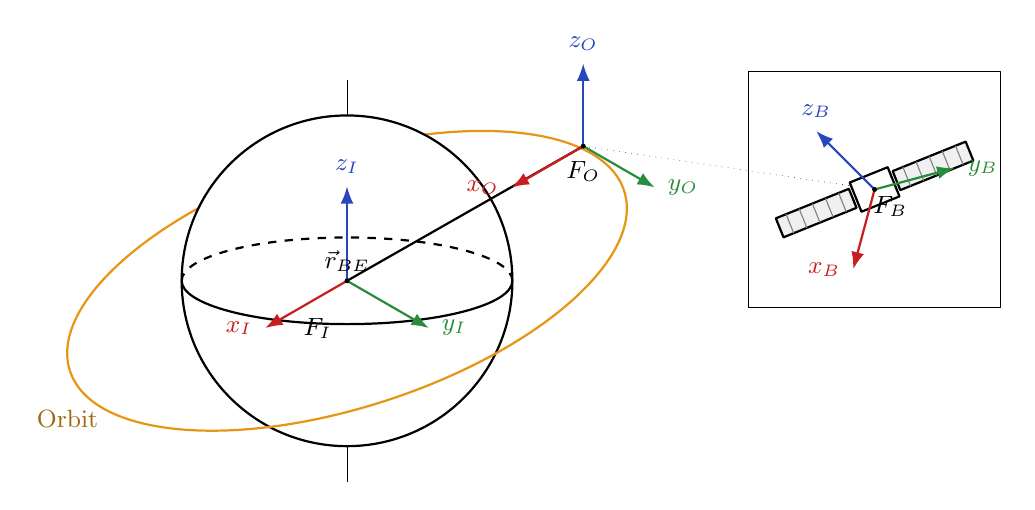
\begin{tikzpicture}[>=Latex, line join=round]

% ============ ORBIT: back half (drawn first, so the Earth fill below can hide it) ============
\coordinate (Ecen) at (0,0);
\begin{scope}[rotate=18]
  \draw[orbitorange, thick] (3.7,0) arc (0:180:3.7 and 1.6);
\end{scope}

% ============ EARTH ============
\fill[white] (Ecen) circle (2.1); % opaque disc occludes the part of the orbit passing behind it
\draw[thick] (Ecen) circle (2.1);
% equator: solid front half, dashed back half for a 3D look
\draw[thick, dashed] ($(Ecen)+(2.1,0)$) arc (0:180:2.1 and 0.55);
\draw[thick]         ($(Ecen)+(-2.1,0)$) arc (180:360:2.1 and 0.55);
\draw[very thin] (0,-2.1) -- (0,-2.55);
\draw[very thin] (0,2.1) -- (0,2.55);

% inertial frame triad at earth centre
\triad{Ecen}{1.2}{I}
\node[anchor=north east,xshift=-2pt,yshift=-10pt] at (Ecen) {\small $F_I$};

% ============ ORBIT: front half (drawn after Earth, so it stays visible on top) ============
\begin{scope}[rotate=18]
  \draw[orbitorange, thick] (-3.7,0) arc (180:360:3.7 and 1.6);
\end{scope}

\node[orbitorange!70!black] at ($(Ecen)+(-3.55,-1.75)$) {\small Orbit};

% ---- point on the orbit where the orbit frame lives ----
\coordinate (OrbPt) at ($(Ecen)+(3.0,1.71)$);

% radius vector from earth centre to the orbit point
\draw[thick] (Ecen) -- (OrbPt);
\node[sloped, above, pos=1.22] at ($(Ecen)!1.22!(OrbPt)$) {\small $\vec{r}_{BE}$}; %{\small $[\bm{R}]^{OI},\ [\bm{t}]^{OI}$}

\triad{OrbPt}{1.05}{O}
\node[below=2pt] at (OrbPt) {\small $F_O$};

% velocity vector, tangent to the orbit at the orbit point
% \draw[-{Latex[length=2.4mm]}, black, thick] (OrbPt) -- ++(0:1.4) node[right] {\small $\vec{v}$};

% ============ SATELLITE + BODY FRAME (offset from O for clarity, as in ref.) ============
\coordinate (Sat) at ($(OrbPt)+(3.7,-0.55)$);
\draw[very thin, dotted] (OrbPt) -- (Sat);

% zoom call-out box (kept axis-aligned, not rotated with the satellite)
\begin{scope}[shift=(Sat)]
  \draw[solid] (-1.6,-1.5) rectangle (1.6,1.5);
\end{scope}

\begin{scope}[shift=(Sat), rotate=22]
  % bus
  \draw[thick, fill=white] (-0.26,-0.20) rectangle (0.26,0.20);
  % solar panels
  \draw[thick, fill=gray!12] (-1.30,-0.13) rectangle (-0.30,0.13);
  \draw[thick, fill=gray!12] (0.30,-0.13) rectangle (1.30,0.13);
  \foreach \x in {-1.16,-0.98,-0.80,-0.62,-0.44}
    \draw[gray] (\x,-0.13) -- (\x,0.13);
  \foreach \x in {0.44,0.62,0.80,0.98,1.16}
    \draw[gray] (\x,-0.13) -- (\x,0.13);
\end{scope}
\begin{scope}[rotate around={45:(Sat)}]
\triad{Sat}{1.05}{B}
\end{scope}
\node[anchor=north west,xshift=-4pt,yshift=1pt] at (Sat) {\small $F_B$};
\end{tikzpicture}
\caption{Diagram showing the Earth, orbit and satellite with the relevant reference frames.}
\label{fig:reference_frames}
\end{figure}
